%%% RESULTS %%%
\section{Results} \label{sec:results}

\paragraph{Relative error and residual norms of singular triplets}

The relative error and residual norm of the leading $k=50$ singular triplets for the CRAN dataset at $\phi=1,5,10$ using Algorithms 2.1, 2.2, and \verb|FrequentDirections| are shown in Figure \ref{fig:cran_relerr_resnorm}.
Due to the large number of figures, the complete set of plots for the standard experiments are presented in Sections A to E in the Supplementary Materials.
When comparing the relative error and residual norm plots for Algorithm 2.1 on CRAN, CISI, and MED, our results matched those of \cite{Kalantzis2021} exactly.
For Algorithm 2.2, the plots did not match exactly, though the differences never exceeded half an order of magnitude and are attributable to the randomness inherent in Algorithm 2.2. 

\begin{figure}[h]
  \centering
  \begin{subfigure}[b]{0.32\textwidth}
    \centering
    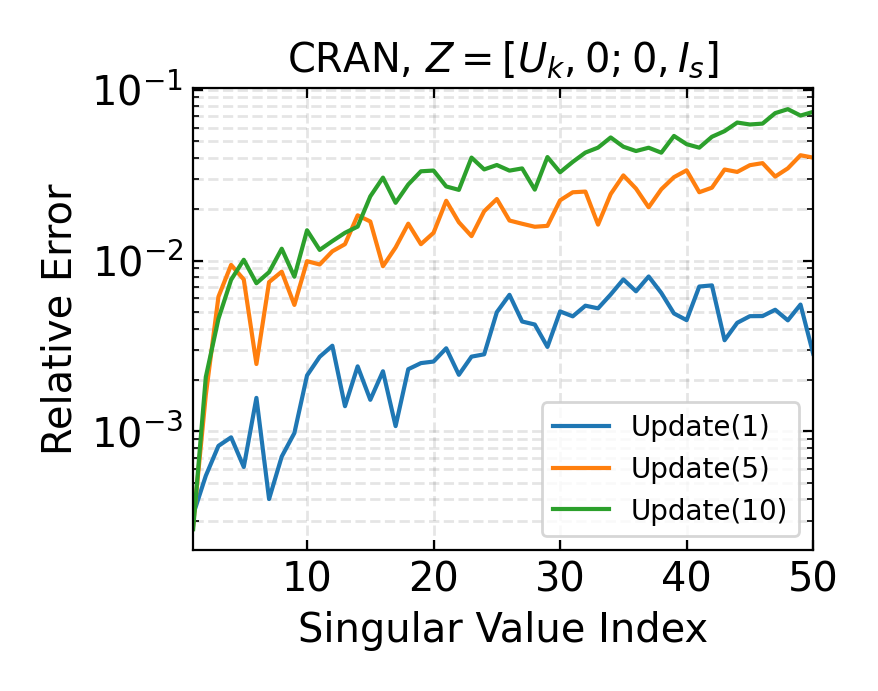
\includegraphics[width=\textwidth]{../openreview/figures/report_figures/CRAN_zha-simon_n_batches_10_k_dims_50_rel_err.png}
    \caption{CRAN relative error (Alg. 2.1)}
  \end{subfigure}
  \hfill
  \begin{subfigure}[b]{0.32\textwidth}
    \centering
    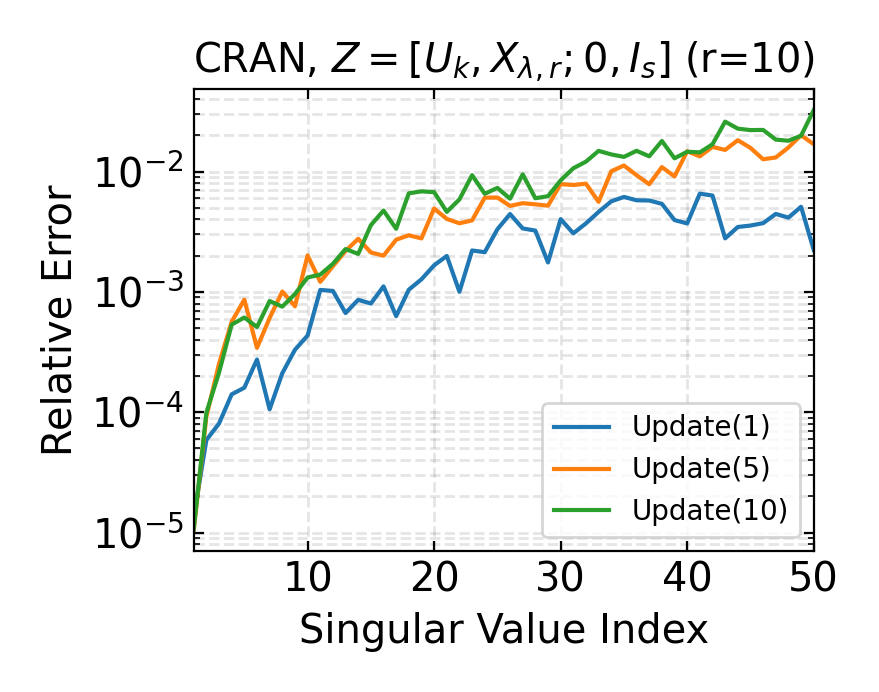
\includegraphics[width=\textwidth]{../openreview/figures/report_figures/CRAN_bcg_n_batches_10_k_dims_50_rval_10_rel_err.png}
    \caption{CRAN relative error (Alg. 2.2)}
  \end{subfigure}
  \hfill
  \begin{subfigure}[b]{0.32\textwidth}
    \centering
    \includegraphics[width=\textwidth]{../openreview/figures/report_figures/CRAN_frequent-directions_n_batches_10_k_dims_50_rel_err.png}
    \caption{CRAN relative error (FD)}
    \label{fig:cran_rel_err_fd}
  \end{subfigure}
  %
  \begin{subfigure}[b]{0.32\textwidth}
    \centering
    \includegraphics[width=\textwidth]{../openreview/figures/report_figures/CRAN_zha-simon_n_batches_10_k_dims_50_res_norm.png}
    \caption{CRAN residual norm (Alg. 2.1)}
  \end{subfigure}
  \hfill
  \begin{subfigure}[b]{0.32\textwidth}
    \centering
    \includegraphics[width=\textwidth]{../openreview/figures/report_figures/CRAN_bcg_n_batches_10_k_dims_50_rval_10_res_norm.png}
    \caption{CRAN residual norm (Alg. 2.2)}
  \end{subfigure}
  \hfill
  \begin{subfigure}[b]{0.32\textwidth}
    \centering
    \includegraphics[width=\textwidth]{../openreview/figures/report_figures/CRAN_frequent-directions_n_batches_10_k_dims_50_res_norm.png}
    \caption{CRAN residual norm (FD)}
    \label{fig:cran_res_norm_fd}
  \end{subfigure}
  \caption{Relative errors and residual norms at $\phi=1,5,10$ for CRAN with Algorithm 2.1, Algorithm 2.2, and FD.}
  \label{fig:cran_relerr_resnorm}
\end{figure}


Our comparison of the relative error and residual norm of the $k=50$-th singular triplet for Algorithm 2.2 with various values of $r$ revealed a similar result to \cite{Kalantzis2021} – across the three methods, Algorithm 2.2 had the lowest errors, and within variations of Algorithm 2.2, larger values of $r$ yielded higher accuracy.

\begin{table}[h]
\centering
\begin{tabular}{@{}cccccccc@{}}
\toprule

& \multicolumn{3}{c}{\textbf{MED}} & \multicolumn{2}{c}{\textbf{CRAN}} & \multicolumn{2}{c}{\textbf{CISI}} \\ 
\midrule

&    $r$ &      err. &      res. &      err. &      res. &      err. &      res. \\

& \cc 10 & \cc 0.037 & \cc 0.204 & \cc 0.031 & \cc 0.174 & \cc 0.038 & \cc 0.224 \\

&     20 &     0.028 &     0.172 &     0.021 &     0.144 &     0.019 &     0.149 \\

& \cc 30 & \cc 0.021 & \cc 0.154 & \cc 0.012 & \cc 0.113 & \cc 0.014 & \cc 0.119 \\

&     40 &     0.015 &     0.133 &     0.010 &     0.107 &     0.011 &     0.105 \\

\multirow{-5}{*}
{\begin{tabular}[c]{@{}c@{}}
$Z=\begin{pmatrix} U_k & X_{\lambda,r} & \\ & & I_s \end{pmatrix}$
\end{tabular}} 

& \cc 50 & \cc 0.013 & \cc 0.121 & \cc 0.008 & \cc 0.097 & \cc 0.009 & \cc 0.096 \\ 
\midrule

\begin{tabular}[c]{@{}c@{}}
$Z=\begin{pmatrix} U_k & \\ & I_s
\end{pmatrix}$\end{tabular}

& – & 0.101 & 0.294 & 0.074 & 0.295 & 0.080 & 0.382 \\ 
\midrule

FrequentDirections

& – & 0.212 & 1.031 & 0.216 & 1.045 & 0.205 & 1.032 \\ 
\bottomrule
\end{tabular}
\caption{Relative error and residual norm of approximation of the singular triplet $(\huj{50}, \hvj{50}, \hsigj{50})$}
\label{tab:err_res_50}
\end{table}

\paragraph{Runtime}

For all three of the datasets which we measured runtimes on, we found Algorithm 2.2 to require a substantially longer amount of time to complete all of its updates.
Algorithm 2.1 and \verb|FrequentDirections| required a similar length of time, though Algorithm 2.1 was consistently faster than \verb|FrequentDirections| by a small margin.
The runtime plots for the standard experiments are shown in Section F of the Supplementary Materials. 

\begin{figure}[h]
  \centering
  \begin{subfigure}[b]{0.49\textwidth}
    \centering
    \includegraphics[width=\textwidth]{../openreview/figures/report_figures/CRAN_runtimes_batch_split_10.png}
    \caption{Runtime vs. $k$}
  \end{subfigure}
  \hfill
  \begin{subfigure}[b]{0.49\textwidth}
    \centering
    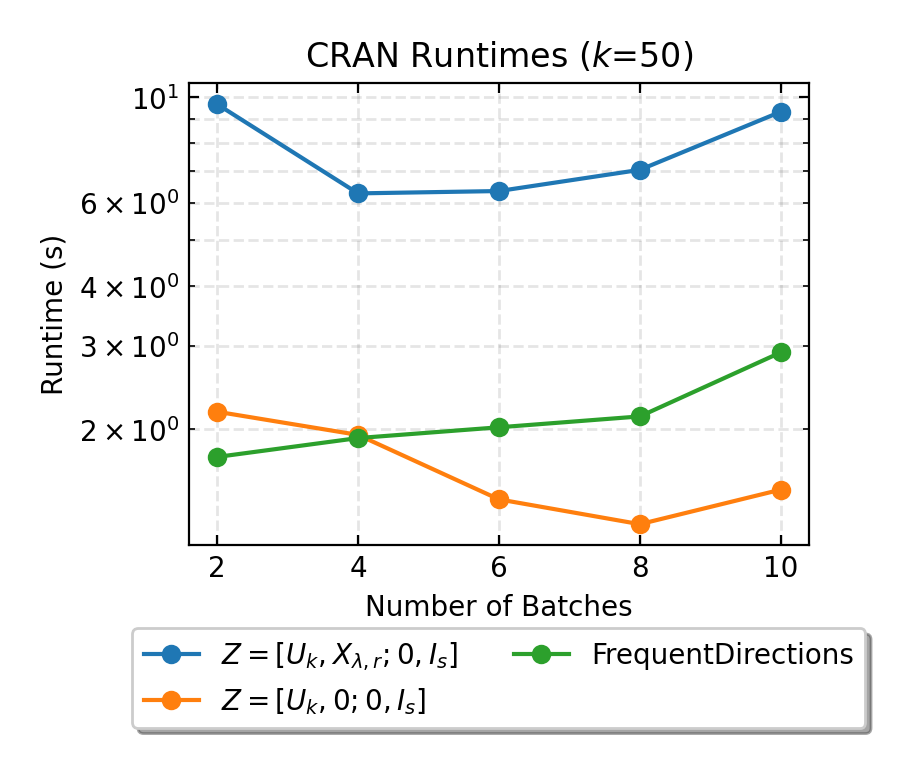
\includegraphics[width=\textwidth]{../openreview/figures/report_figures/CRAN_runtimes_k_dim_50.png}
    \caption{Runtime vs. number of batches}
  \end{subfigure}
  \caption{CRAN runtimes as a function of rank $k$ (left) and number of batch splits (right).}
  \label{fig:cran_runtime}
\end{figure}


\paragraph{Number of batches and rank} 

Due to space-related constraints, we chose to only include two examples from the array of plots generated (Figure \ref{fig:cran_variations}).
Despite the large variation in the parameters, we can see that the residual norm for overlapping update numbers and $k$ share very similar values.

\begin{figure}[h]
  \centering
  \begin{subfigure}[b]{0.49\textwidth}
    \centering
    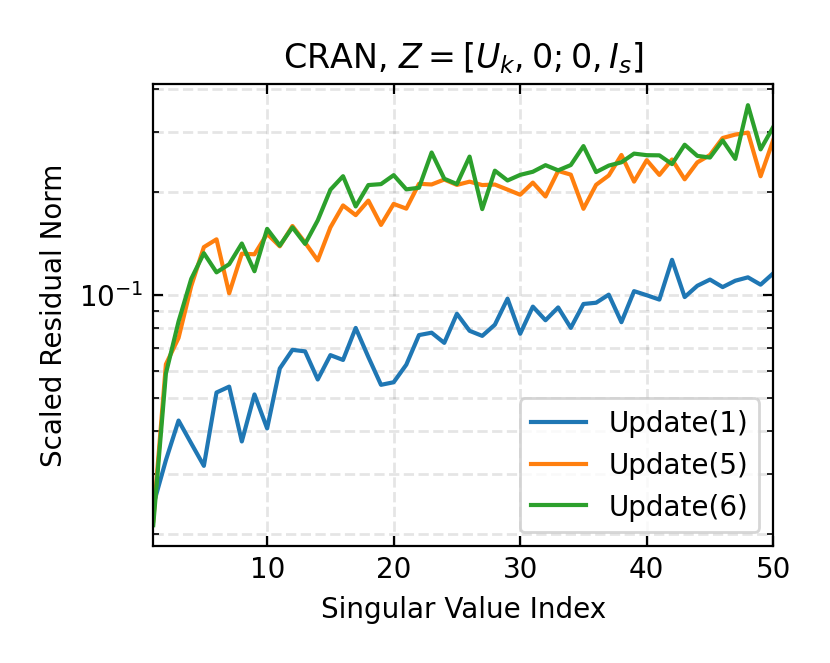
\includegraphics[width=\textwidth]{../openreview/figures/report_figures/CRAN_zha-simon_n_batches_6_k_dims_50_res_norm.png}
    \caption{6 batches, $k=50$}
  \end{subfigure}
  \hfill
  \begin{subfigure}[b]{0.49\textwidth}
    \centering
    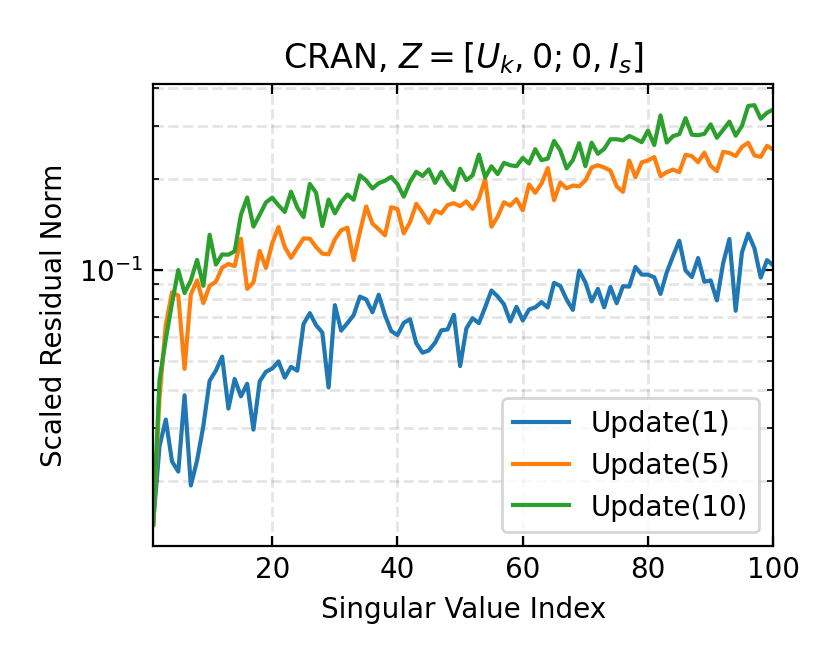
\includegraphics[width=\textwidth]{../openreview/figures/report_figures/CRAN_zha-simon_n_batches_10_k_dims_100_res_norm.png}
    \caption{10 batches, $k=100$}
  \end{subfigure}
  \caption{Examples of residual norm for experimental parameters outside of what was investigated by \cite{Kalantzis2021}.}
  \label{fig:cran_variations}
\end{figure}


